\documentclass[aspectratio=169,11pt]{beamer}
\usetheme{Madrid}
\usecolortheme{seahorse}
\usefonttheme{professionalfonts}

\usepackage{amsmath,amssymb,bm}
\usepackage{booktabs}
\usepackage{array}
\usepackage{tikz}
\usetikzlibrary{positioning,arrows.meta,shapes.geometric}
\usepackage{listings}
\usepackage{xcolor}
\usepackage{xeCJK}
\usepackage{fontspec}
\usepackage{hyperref}

\setmainfont{texgyreheros-regular.otf}[BoldFont=texgyreheros-bold.otf,ItalicFont=texgyreheros-italic.otf]
\setsansfont{texgyreheros-regular.otf}[BoldFont=texgyreheros-bold.otf,ItalicFont=texgyreheros-italic.otf]
\setmonofont{lmmono10-regular.otf}[BoldFont=lmmonolt10-bold.otf]
\setCJKmainfont{FandolHei-Regular.otf}
\setCJKsansfont{FandolHei-Regular.otf}
\setCJKmonofont{FandolFang-Regular.otf}

\definecolor{myblue}{RGB}{36,88,135}
\definecolor{mygreen}{RGB}{40,120,80}
\definecolor{myred}{RGB}{150,45,45}
\definecolor{mygray}{RGB}{90,90,90}
\definecolor{myorange}{RGB}{190,110,35}
\setbeamercolor{title}{fg=myblue}
\setbeamercolor{frametitle}{fg=myblue}
\setbeamercolor{structure}{fg=myblue}
\setbeamertemplate{navigation symbols}{}
\setbeamertemplate{footline}[frame number]

\lstset{
  basicstyle=\ttfamily\scriptsize,
  keywordstyle=\color{myblue}\bfseries,
  stringstyle=\color{mygreen},
  commentstyle=\color{mygray},
  breaklines=true,
  frame=single,
  columns=fullflexible,
  keepspaces=true,
  showstringspaces=false
}

\newcommand{\Rplus}{\mathbb{R}_{+}}
\newcommand{\relu}[1]{\left[#1\right]_{+}}

\title[Week 4]{Week 4: 三相 N-1 扫描与 Violation Label 设计}
\subtitle{Three-phase N-1 security labeling for microgrid AI screening}
\author{ECE Course: Physics-informed AI for Microgrid Security Prediction}
\date{}

\begin{document}

\begin{frame}
  \titlepage
\end{frame}

\begin{frame}{本周学习目标}
\begin{enumerate}
  \item 把 Week 3 的 base-case scenarios $x_t$ 扩展成 N-1 samples $(x_t,c_k)$。
  \item 建立 contingency catalog: line outage, PV trip, BESS trip, PCC outage。
  \item 设计 phase-aware violation labels: voltage, current/loading, VUF, service loss, convergence。
  \item 定义 severity score，用于 Week 5/7 的分类、回归和 ranking。
  \item 手写 \texttt{runpp\_3ph()} based scanning loop，并证明每次 contingency 后状态可恢复。
  \item 导出 AI-ready dataset，并用 validation suite 检查正确性。
\end{enumerate}
\end{frame}

\begin{frame}[shrink=4]{八周课程中的位置}
\centering
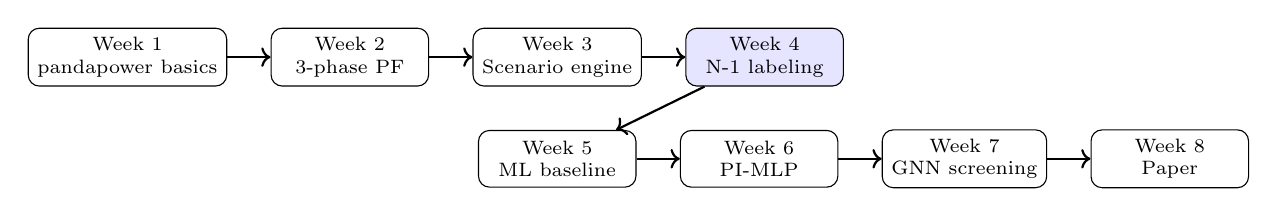
\begin{tikzpicture}[node distance=0.55cm, every node/.style={font=\scriptsize}]
\tikzstyle{box}=[draw, rounded corners, minimum width=2.0cm, minimum height=0.72cm, align=center]
\node[box] (w1) {Week 1\\pandapower basics};
\node[box, right=of w1] (w2) {Week 2\\3-phase PF};
\node[box, right=of w2] (w3) {Week 3\\Scenario engine};
\node[box, right=of w3, fill=blue!10] (w4) {Week 4\\N-1 labeling};
\node[box, below=of w3] (w5) {Week 5\\ML baseline};
\node[box, right=of w5] (w6) {Week 6\\PI-MLP};
\node[box, right=of w6] (w7) {Week 7\\GNN screening};
\node[box, right=of w7] (w8) {Week 8\\Paper};
\draw[->, thick] (w1)--(w2);
\draw[->, thick] (w2)--(w3);
\draw[->, thick] (w3)--(w4);
\draw[->, thick] (w4)--(w5);
\draw[->, thick] (w5)--(w6);
\draw[->, thick] (w6)--(w7);
\draw[->, thick] (w7)--(w8);
\end{tikzpicture}
\vspace{0.4cm}

\begin{block}{Week 4 的地位}
Week 4 是整个 AI 安全预测项目的数据根基：标签错了，后面的模型越强，结论越危险。
\end{block}
\end{frame}

\begin{frame}{从 Week 3 到 Week 4}
\begin{columns}
\begin{column}{0.48\textwidth}
\textbf{Week 3 输出}\
\[
\mathcal{D}_{base}=\{x_t\}_{t=1}^{T}
\]
\begin{itemize}
  \item load scale
  \item phase imbalance factors
  \item PV scale
  \item BESS setpoint
  \item base-case three-phase PF metrics
\end{itemize}
\end{column}
\begin{column}{0.48\textwidth}
\textbf{Week 4 输出}\
\[
\mathcal{D}_{N-1}=\{(x_t,c_k,y_{t,k},s_{t,k})\}
\]
\begin{itemize}
  \item contingency metadata
  \item post-contingency metrics
  \item violation type flags
  \item binary label
  \item severity score
\end{itemize}
\end{column}
\end{columns}
\end{frame}

\begin{frame}{为什么 label 设计是科研核心？}
\begin{block}{AI 模型真正学习什么？}
\[
f_\theta(x_t,c_k) \approx y_{t,k},\; s_{t,k}
\]
\end{block}
\begin{itemize}
  \item 如果 $y_{t,k}$ 只表示电压越限，模型不会学习 service interruption。
  \item 如果 severity 没有区分 critical load loss，模型的 ranking 会忽略真正危险的 outage。
  \item 如果 non-convergence 被直接丢弃，模型会低估极端 contingency 的风险。
\end{itemize}
\begin{alertblock}{本周原则}
宁可标签偏保守，也不要让危险 contingency 被误标为 safe。
\end{alertblock}
\end{frame}

\begin{frame}{三相微电网 N-1 为什么更复杂？}
\begin{columns}
\begin{column}{0.48\textwidth}
\textbf{常规 transmission N-1}\
\begin{itemize}
  \item bus voltage violation
  \item line / transformer thermal overload
  \item PF non-convergence
\end{itemize}
\end{column}
\begin{column}{0.48\textwidth}
\textbf{三相 microgrid / LV feeder}\
\begin{itemize}
  \item per-phase voltage violation
  \item per-phase current/loading violation
  \item voltage unbalance factor, VUF
  \item radial feeder service interruption
  \item single-phase PV/BESS effects
  \item PCC outage / no slack source
\end{itemize}
\end{column}
\end{columns}
\vspace{0.2cm}
\begin{block}{关键变化}
N-1 不只是“设备越限”，还包括“部分负荷没有供电”。
\end{block}
\end{frame}

\begin{frame}{Week 4 的 teaching feeder}
\centering
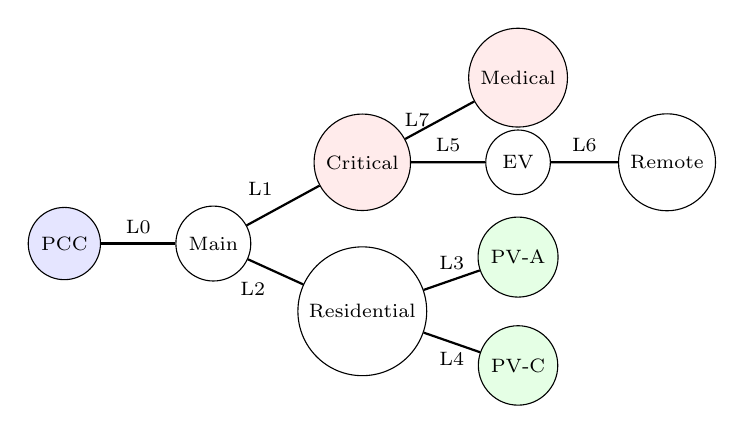
\begin{tikzpicture}[scale=0.86, every node/.style={font=\scriptsize}]
\tikzstyle{bus}=[draw, circle, minimum size=0.82cm, align=center]
\node[bus, fill=blue!10] (pcc) at (0,0) {PCC};
\node[bus] (main) at (2.2,0) {Main};
\node[bus, fill=red!8] (crit) at (4.4,1.2) {Critical};
\node[bus] (res) at (4.4,-1.0) {Residential};
\node[bus, fill=green!10] (pva) at (6.7,-0.2) {PV-A};
\node[bus, fill=green!10] (pvc) at (6.7,-1.8) {PV-C};
\node[bus] (ev) at (6.7,1.2) {EV};
\node[bus] (remote) at (8.9,1.2) {Remote};
\node[bus, fill=red!8] (med) at (6.7,2.45) {Medical};
\draw[thick] (pcc)--node[above]{L0} (main);
\draw[thick] (main)--node[above left]{L1} (crit);
\draw[thick] (main)--node[below left]{L2} (res);
\draw[thick] (res)--node[above]{L3} (pva);
\draw[thick] (res)--node[below]{L4} (pvc);
\draw[thick] (crit)--node[above]{L5} (ev);
\draw[thick] (ev)--node[above]{L6} (remote);
\draw[thick] (crit)--node[left]{L7} (med);
\end{tikzpicture}
\vspace{0.2cm}

\small 9 buses, 8 lines, radial, asymmetric loads, single-phase PV, BESS-like static setpoint.
\end{frame}

\begin{frame}{Contingency 的数学定义}
\begin{block}{N-1 contingency catalog}
\[
c_k \in \mathcal{C},\quad k=1,\ldots,K
\]
每个 $c_k$ 表示一个单一设备或单一功能退出事件。
\end{block}
\begin{itemize}
  \item Week 4 MVP: line outage, PV trip, BESS trip, PCC outage。
  \item 每个 $c_k$ 必须能映射回 pandapower input table。
  \item 每个 $c_k$ 只能改变输入状态，不应直接修改结果表。
\end{itemize}
\begin{exampleblock}{本 notebook}
7 scenarios $\times$ 11 contingencies = 77 N-1 samples.
\end{exampleblock}
\end{frame}

\begin{frame}{Contingency catalog schema}
\scriptsize
\begin{tabular}{llp{6.2cm}}
\toprule
字段 & 类型 & 作用 \\
\midrule
\texttt{contingency\_id} & string & 唯一 ID，例如 \texttt{line\_1\_out} \\
\texttt{contingency\_type} & string & \texttt{line\_outage}, \texttt{pv\_trip}, \texttt{bess\_trip}, \texttt{pcc\_outage} \\
\texttt{element\_table} & string & 指向 pandapower input table \\
\texttt{element\_index} & int/string & 指向具体设备编号 \\
\texttt{element\_name} & string & 人可读设备名 \\
\texttt{description} & string & 教学/报告解释 \\
\bottomrule
\end{tabular}
\vspace{0.3cm}

\begin{block}{Proof check}
检查 catalog 是否 ID 唯一、类型合法、设备索引真实存在。
\end{block}
\end{frame}

\begin{frame}{Line outage: radial feeder 的特殊问题}
\begin{columns}
\begin{column}{0.52\textwidth}
\begin{itemize}
  \item 线路退出可能不只是改变潮流。
  \item 在 radial feeder 中，线路退出会切断下游 buses。
  \item 下游 load 可能没有供电，即使剩余网络仍然收敛。
\end{itemize}
\begin{block}{Topology label}
\[
\mathcal{N}_{off}=\mathcal{N}\setminus \mathcal{N}_{reachable(PCC)}
\]
\end{block}
\end{column}
\begin{column}{0.43\textwidth}
\centering
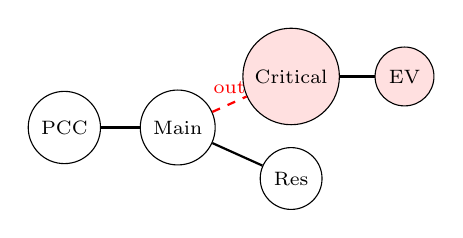
\begin{tikzpicture}[scale=0.72, every node/.style={font=\scriptsize}]
\node[draw, circle] (pcc) at (0,0) {PCC};
\node[draw, circle] (main) at (2,0) {Main};
\node[draw, circle, fill=red!12] (crit) at (4,0.9) {Critical};
\node[draw, circle, fill=red!12] (ev) at (6,0.9) {EV};
\node[draw, circle] (res) at (4,-0.9) {Res};
\draw[thick] (pcc)--(main);
\draw[thick, red, dashed] (main)--node[above]{out} (crit);
\draw[thick] (crit)--(ev);
\draw[thick] (main)--(res);
\end{tikzpicture}
\end{column}
\end{columns}
\end{frame}

\begin{frame}[fragile]{PV trip: 单相 DER 的影响}
\begin{itemize}
  \item PV trip 设置相应 \texttt{asymmetric\_sgen.in\_service=False}。
  \item 单相 PV 退出会改变相别功率平衡。
  \item 高 PV 场景下，PV trip 可能降低过电压风险，也可能提高 PCC import。
\end{itemize}
\begin{block}{教学问题}
PV trip 不一定总是 dangerous；它也可能让某些 high-PV operating point 更接近正常电压。
\end{block}
\begin{lstlisting}[language=Python]
if ctype == "pv_trip":
    net.asymmetric_sgen.loc[element_index, "in_service"] = False
\end{lstlisting}
\end{frame}

\begin{frame}[fragile]{BESS trip: 静态 setpoint 的退出}
\begin{itemize}
  \item Week 4 的 BESS 仍是 static setpoint，不更新 SOC。
  \item 放电时：BESS 作为 \texttt{asymmetric\_sgen} 注入。
  \item 充电时：BESS 作为 \texttt{asymmetric\_load} 消耗。
  \item BESS trip 要同时关闭 charge placeholder 和 discharge placeholder。
\end{itemize}
\begin{lstlisting}[language=Python]
elif ctype == "bess_trip":
    discharge_sgen.in_service = False
    charge_load.in_service = False
\end{lstlisting}
\begin{alertblock}{符号提醒}
Notebook 采用课程约定：$P^{BESS}_{dis}>0$ 表示放电注入，$P^{BESS}_{dis}<0$ 表示充电消耗。
\end{alertblock}
\end{frame}

\begin{frame}{PCC outage: no-slack source}
\begin{itemize}
  \item PCC outage 在 grid-connected MVP 中表示与上级电网断开。
  \item 如果没有 islanded grid-forming source，则三相潮流没有 slack source。
  \item Notebook 对这种情况不强行运行潮流，而是保守标记为 non-convergence violation。
\end{itemize}
\begin{block}{保守标签}
\[
y_C=1 \quad \text{if no in-service slack source exists}
\]
\end{block}
\begin{exampleblock}{后续扩展}
Week 4 暂不建模 islanded mode。后续可加入 grid-forming BESS 或 diesel generator。
\end{exampleblock}
\end{frame}

\begin{frame}{Violation taxonomy}
\scriptsize
\begin{tabular}{lll}
\toprule
标签 & 来源 & 工程含义 \\
\midrule
\texttt{voltage\_low\_violation} & \texttt{res\_bus\_3ph} & 任一相电压低于下限 \\
\texttt{voltage\_high\_violation} & \texttt{res\_bus\_3ph} & 任一相电压高于上限 \\
\texttt{loading\_violation} & \texttt{res\_line\_3ph} & 任一线路/相 loading 超过限值 \\
\texttt{vuf\_violation} & 对称分量或结果表 & 电压不平衡因子超过限值 \\
\texttt{non\_convergence\_violation} & solver / no slack & 三相潮流不可用或不收敛 \\
\texttt{service\_loss\_violation} & graph topology & 负荷从 PCC 断开 \\
\texttt{critical\_service\_loss\_violation} & graph + load name & 重要负荷没有供电 \\
\bottomrule
\end{tabular}
\vspace{0.3cm}

\begin{block}{Binary label}
\[
y=\bigvee_m y_m
\]
\end{block}
\end{frame}

\begin{frame}{相电压越限标签}
\begin{block}{Per-phase voltage bounds}
\[
V^{min}\le |V_{i,\phi}| \le V^{max},\quad \phi\in\{a,b,c\}
\]
\end{block}
\begin{align*}
y_{V,low}&=\mathbb{I}\left(\min_{i,\phi}|V_{i,\phi}|<V^{min}\right)\\
y_{V,high}&=\mathbb{I}\left(\max_{i,\phi}|V_{i,\phi}|>V^{max}\right)
\end{align*}
\begin{itemize}
  \item Week 4 teaching thresholds: $V^{min}=0.95$, $V^{max}=1.05$ p.u.
  \item 三相系统必须检查每一相，而不是只检查正序或平均电压。
\end{itemize}
\end{frame}

\begin{frame}{线路 loading / current 越限标签}
\begin{block}{Per-phase loading}
\[
I_{\ell,eff}^{max}=I_\ell^{max}df_\ell n_{\ell,parallel},\qquad
loading_{\ell,\phi}=100\frac{|I_{\ell,\phi}|}{I^{max}_{\ell,eff}}
\]
\end{block}
\[
y_I=\mathbb{I}\left(\max_{\ell,\phi} loading_{\ell,\phi} > 100\%\right)
\]
\begin{itemize}
  \item Notebook 使用 \texttt{res\_line\_3ph} 中的 loading columns。
  \item 同时提供手算 proof：用 \texttt{max\_i\_ka} 复核 loading percent。
\end{itemize}
\end{frame}

\begin{frame}{VUF 标签}
\begin{block}{对称分量定义}
\[
V^{(1)}=\frac{1}{3}\left(V_a+aV_b+a^2V_c\right),\quad
V^{(2)}=\frac{1}{3}\left(V_a+a^2V_b+aV_c\right)
\]
\[
\mathrm{VUF}=100\frac{|V^{(2)}|}{|V^{(1)}|}
\]
\end{block}
\begin{itemize}
  \item Week 4 教学阈值：$\mathrm{VUF}^{max}=2\%$，与 Week 2/6 保持一致。
  \item Notebook 可从 \texttt{vm\_a\_pu}, \texttt{va\_a\_degree} 等字段手算 VUF。
  \item 本周数据中 VUF 没有超过阈值，但保留标签用于后续 full feeder 实验。
\end{itemize}
\end{frame}

\begin{frame}{Service-loss 标签}
\begin{block}{Topology-based service interruption}
\[
P_{unserved}=\sum_{i\notin\mathcal{N}_{reachable(PCC)}} P_{load,i}
\]
\[
y_S=\mathbb{I}(P_{unserved}>\epsilon)
\]
\end{block}
\begin{itemize}
  \item 这不是 power-flow metric，而是 graph connectivity metric。
  \item 即使剩余网络电压正常，下游负荷被切除也必须标为 unsafe。
  \item 对 microgrid / radial LV feeder 尤其重要。
\end{itemize}
\end{frame}

\begin{frame}{Critical service-loss 标签}
\begin{block}{重要负荷未供电}
\[
y_{S,crit}=\mathbb{I}(P_{critical,unserved}>\epsilon)
\]
\end{block}
\begin{itemize}
  \item Critical load 和 medical load 的 outage 应比普通 residential load 更严重。
  \item Notebook 同时保存 \texttt{unserved\_load\_mw} 和 \texttt{critical\_unserved\_load\_mw}。
  \item 后续 AI ranking 可以优先排序 critical-load interruption。
\end{itemize}
\begin{alertblock}{论文写作提醒}
Severity 设计必须解释工程理由，不能只是数学上方便。
\end{alertblock}
\end{frame}

\begin{frame}{Severity score 设计}
\small
\begin{align*}
s(x_t,c)&=\max\{s_V^{low},s_V^{high},s_I,s_U,s_C,s_S,s_{S,crit}\}\\
s_V^{low}&=\relu{\frac{V^{min}-V_{min}}{V^{min}}}\\
s_V^{high}&=\relu{\frac{V_{max}-V^{max}}{V^{max}}}\\
s_I&=\relu{\frac{loading_{max}}{100}-1}\\
s_U&=\relu{\frac{VUF_{max}}{VUF^{max}}-1}
\end{align*}
\begin{itemize}
  \item Non-convergence severity is set to 1.
  \item Service loss severity is normalized by a teaching-scale load base.
\end{itemize}
\end{frame}

\begin{frame}{Binary label 与 multi-label 同时保存}
\begin{columns}
\begin{column}{0.5\textwidth}
\textbf{Binary label}\
\[
y=\mathbb{I}(s>0)
\]
\begin{itemize}
  \item Week 5 classification
  \item high-recall screening
  \item false negative analysis
\end{itemize}
\end{column}
\begin{column}{0.5\textwidth}
\textbf{Multi-label flags}\
\begin{itemize}
  \item voltage low / high
  \item loading
  \item VUF
  \item service loss
  \item critical service loss
  \item non-convergence
\end{itemize}
\end{column}
\end{columns}
\begin{block}{为什么都要保存？}
Binary label 训练简单；multi-label flags 用于 error analysis、ablation 和论文解释。
\end{block}
\end{frame}

\begin{frame}[fragile]{手写 N-1 scanning loop}
\begin{lstlisting}[language=Python]
for scenario in scenarios:
    reset_input_state(net)
    apply_scenario(net, scenario)

    for contingency in contingencies:
        reset_input_state(net)
        apply_scenario(net, scenario)
        scenario_signature = input_signature(net)

        apply_contingency(net, contingency)
        service = detect_unserved_load(net)
        converged = run_three_phase_power_flow(net)
        metrics = extract_post_contingency_metrics(net)
        labels = label_from_metrics(metrics, service)

        restore_and_assert_signature(net, scenario_signature)
        save_row(...)
\end{lstlisting}
\end{frame}

\begin{frame}{为什么不用内置 contingency 就结束？}
\begin{itemize}
  \item 本项目需要支持 PV trip, BESS trip, PCC outage。
  \item 需要保存 service interruption，而不是只保存电压/线路 loading。
  \item 需要自定义 phase-aware severity score。
  \item 需要把每个样本直接导出为 AI training row。
\end{itemize}
\begin{block}{本周目标}
不是否定工具内置功能，而是构造一个适合微电网 AI 研究的透明数据生成器。
\end{block}
\end{frame}

\begin{frame}{Proof 1: input network integrity}
\begin{itemize}
  \item 所有 line / load / sgen / ext-grid 的 bus index 必须存在。
  \item line length 和 current rating 必须为正。
  \item 三相潮流需要 zero-sequence line parameters。
  \item teaching feeder 必须连通且径向。
  \item PV 和 BESS metadata 必须能映射回 pandapower 表。
\end{itemize}
\begin{exampleblock}{Notebook 输出}
9 buses, 8 lines, 6 asymmetric loads, 4 asymmetric sgens; connected and radial checks passed.
\end{exampleblock}
\end{frame}

\begin{frame}{Proof 2: N-0 reference cross-check}
\begin{block}{检查公式}
\[
summary(x_t,\text{no outage})=summary_{base}(x_t)
\]
\end{block}
\begin{itemize}
  \item 对每个 scenario 重新运行 no-outage 三相潮流。
  \item 比较 \texttt{min\_vm\_pu}, \texttt{max\_vm\_pu}, \texttt{max\_vuf\_percent}, loading, PCC import。
  \item 最大误差要求小于数值容差。
\end{itemize}
\begin{alertblock}{能发现什么 bug？}
错误的 reset、错误的 result extraction、或者 scenario application 有隐藏状态污染。
\end{alertblock}
\end{frame}

\begin{frame}{Proof 3: state restoration}
\begin{columns}
\begin{column}{0.55\textwidth}
\begin{itemize}
  \item 每个 contingency 都会修改 input tables。
  \item 如果不恢复，后面的样本会继承前一个 outage。
  \item Notebook 为每个 sample 比较 input signature。
\end{itemize}
\end{column}
\begin{column}{0.43\textwidth}
\begin{block}{Signature check}
\[
\sigma(\text{before})=\sigma(\text{after restore})
\]
\end{block}
\small
\texttt{load P/Q + sgen P/Q + line status + ext-grid status}
\end{column}
\end{columns}
\begin{exampleblock}{Notebook 输出}
\texttt{state\_restoration\_failures = 0}
\end{exampleblock}
\end{frame}

\begin{frame}{Proof 4: service-loss detection}
\begin{itemize}
  \item 构建 in-service line graph。
  \item 找到 PCC 所在 connected component。
  \item 汇总不在该 component 内的负荷。
\end{itemize}
\begin{block}{代表性检查}
\[
\texttt{line\_1\_out}:\quad P_{unserved}=0.052\;\mathrm{MW},\quad P_{crit,unserved}=0.027\;\mathrm{MW}
\]
\end{block}
\begin{itemize}
  \item outage 前：unserved load = 0。
  \item outage 后：下游 critical / EV / remote / medical buses 被切断。
\end{itemize}
\end{frame}

\begin{frame}{Proof 5: label consistency}
\begin{block}{检查公式}
\[
\texttt{violation\_label}=\bigvee_m \texttt{violation\_flag}_m
\]
\[
\texttt{safe}\Rightarrow s=0,\quad \texttt{unsafe}\Rightarrow s>0
\]
\end{block}
\begin{itemize}
  \item 这是监督学习数据的最基本一致性。
  \item 如果失败，Week 5 的 confusion matrix 没有意义。
\end{itemize}
\begin{exampleblock}{Notebook 输出}
30 safe rows, 47 unsafe rows; consistency check passed.
\end{exampleblock}
\end{frame}

\begin{frame}{Proof 6: metric finiteness and no-slack check}
\begin{columns}
\begin{column}{0.48\textwidth}
\textbf{Converged rows}\
\begin{itemize}
  \item voltage metrics must be finite
  \item loading metrics must be finite
  \item VUF metrics must be finite
\end{itemize}
\end{column}
\begin{column}{0.48\textwidth}
\textbf{PCC outage rows}\
\begin{itemize}
  \item one row per scenario
  \item no in-service slack
  \item non-convergence violation = true
\end{itemize}
\end{column}
\end{columns}
\begin{exampleblock}{Notebook 输出}
35 rows run and converge; 35 service-loss rows are skipped before PF; 7 PCC-outage rows are marked no-slack/non-converged.
\end{exampleblock}
\end{frame}

\begin{frame}{Validation suite summary}
\scriptsize
\begin{tabular}{ll}
\toprule
Test & Result \\
\midrule
input network integrity & passed \\
contingency table schema & passed \\
base-case convergence & 7 scenarios passed \\
N-0 reference cross-check & 7 scenarios passed \\
sample count & 77 / 77 samples \\
no duplicate samples & 0 duplicates \\
label consistency & 30 safe, 47 unsafe \\
metric finiteness & 35 solved rows \\
PCC outage no-slack & 7 rows passed \\
line service loss present & 35 line rows with service loss \\
state restoration & 0 failures \\
sentinel reproducibility & 5 sentinel rows passed \\
\bottomrule
\end{tabular}
\end{frame}

\begin{frame}{Week 4 dataset statistics}
\begin{columns}
\begin{column}{0.48\textwidth}
\textbf{Dataset size}\
\begin{itemize}
  \item 7 deterministic scenarios
  \item 11 contingencies
  \item 77 total samples
  \item 47 unsafe, 30 safe
\end{itemize}
\end{column}
\begin{column}{0.48\textwidth}
\textbf{By contingency type}\
\scriptsize
\begin{tabular}{lrr}
\toprule
Type & Safe & Unsafe \\
\midrule
BESS trip & 6 & 1 \\
Line outage & 6 & 36 \\
PCC outage & 0 & 7 \\
PV trip & 18 & 3 \\
\bottomrule
\end{tabular}
\end{column}
\end{columns}
\begin{block}{教学解释}
Line outage 危险样本多，是因为 radial feeder 中很多 line outage 会导致 downstream service loss。
\end{block}
\end{frame}

\begin{frame}{Violation type distribution}
\scriptsize
\begin{tabular}{lrp{6.0cm}}
\toprule
Violation type & Count & 解释 \\
\midrule
voltage low & 5 & stress/unbalance 或特定 outage 下电压跌落 \\
voltage high & 0 & teaching scenarios 未触发过电压 \\
loading & 5 & stress scenario 中部分 line loading 超限 \\
VUF & 0 & VUF 保留为后续 full feeder 标签 \\
non-convergence & 7 & PCC outage 无 slack source \\
service loss & 42 & radial line outage / PCC outage 造成负荷失电 \\
critical service loss & 28 & critical/medical buses 失电 \\
\bottomrule
\end{tabular}
\end{frame}

\begin{frame}{AI-ready dataset schema}
\scriptsize
\begin{tabular}{ll}
\toprule
字段组 & 例子 \\
\midrule
scenario features & \texttt{load\_scale}, \texttt{phase\_b\_factor}, \texttt{pv\_scale}, \texttt{bess\_p\_discharge\_mw} \\
contingency features & \texttt{contingency\_type}, \texttt{element\_table}, \texttt{element\_index} \\
post metrics & \texttt{min\_vm\_pu}, \texttt{max\_loading}, \texttt{max\_vuf}, \texttt{unserved\_load\_mw} \\
labels & violation flags, \texttt{violation\_label}, \texttt{severity\_score} \\
\bottomrule
\end{tabular}
\vspace{0.25cm}

\begin{block}{Week 5 使用方式}
\texttt{week4\_ai\_ready\_dataset.csv} 是原始监督数据源；训练时只能选故障前特征，post metrics 和 labels 只用于监督、评估和作图。
\end{block}
\end{frame}

\begin{frame}{从 Week 4 到 Week 5}
\begin{columns}
\begin{column}{0.5\textwidth}
\textbf{Week 4 provides labels}\
\[
(x_t,c_k)\rightarrow y_{t,k},s_{t,k}
\]
\begin{itemize}
  \item expensive three-phase scan
  \item ground truth generation
  \item verified dataset
\end{itemize}
\end{column}
\begin{column}{0.5\textwidth}
\textbf{Week 5 trains models}\
\[
\hat{y}_{t,k}=f_\theta(x_t,c_k)
\]
\begin{itemize}
  \item logistic regression
  \item random forest
  \item gradient boosting
  \item MLP baseline
\end{itemize}
\end{column}
\end{columns}
\begin{alertblock}{评价重点}
不要只看 accuracy；安全筛查更关心 recall 和 false negative rate。
\end{alertblock}
\end{frame}

\begin{frame}{常见错误与 debugging checklist}
\begin{itemize}
  \item 忘记 reset input tables，导致 outage 累积。
  \item 把 non-converged rows 丢弃，导致危险样本消失。
  \item 只检查 average voltage，漏掉单相越限。
  \item line outage 后只看潮流，不看 downstream service loss。
  \item 把 BESS 充电/放电符号弄反。
  \item 用 random split 导致同一 scenario 的相似样本同时出现在 train/test。
\end{itemize}
\begin{block}{建议}
所有 proof 先通过，再讨论模型结构。
\end{block}
\end{frame}

\begin{frame}{Notebook 课堂流程建议}
\begin{enumerate}
  \item 先运行 input integrity 和 base-case convergence proof。
  \item 手动检查 contingency table，确认每个 element index 指向正确设备。
  \item 用 \texttt{line\_1\_out} 解释 service-loss detection。
  \item 运行 full N-1 scan，观察 77 行数据结构。
  \item 运行 validation suite，要求所有 tests passed。
  \item 打开 label distribution 和 top severe contingencies，讨论是否符合工程直觉。
\end{enumerate}
\end{frame}

\begin{frame}{学生练习}
\begin{enumerate}
  \item 新增 \texttt{line\_4\_out} contingency，观察 PV-C lateral outage 是否产生 service-loss label。
  \item 把 $V^{min}$ 从 0.95 改成 0.97，观察 unsafe 样本数量如何变化。
  \item 把 $VUF^{max}$ 从 2\% 改成 1\%，观察 VUF label 是否出现。
  \item 新增 \texttt{single\_pv\_all\_trip} contingency，一次切除所有 PV，并解释这是否仍是 N-1。
  \item 设计一个更合理的 critical-load severity weighting。
\end{enumerate}
\end{frame}

\begin{frame}{科研故事线中的 Week 4}
\begin{block}{论文中的 Dataset Generation Section}
Week 4 对应论文中的 ground-truth label generation pipeline。
\end{block}
\begin{itemize}
  \item 说明三相潮流 ground truth 来自 pandapower \texttt{runpp\_3ph()}。
  \item 说明 contingency catalog 的范围。
  \item 给出 voltage/current/VUF/service/convergence labels。
  \item 给出 severity score。
  \item 报告 dataset statistics 和 validation checks。
\end{itemize}
\end{frame}

\begin{frame}{本周小结}
\begin{enumerate}
  \item Week 4 把 base-case scenario 扩展成 N-1 supervised learning dataset。
  \item 三相 microgrid label 必须同时考虑 electrical violation 和 topology-based service loss。
  \item Severity score 是后续 ranking 和 high-recall screening 的基础。
  \item Validation suite 是科研可信度的一部分，不是代码附属品。
  \item 下一步：使用 \texttt{week4\_ai\_ready\_dataset.csv} 训练 Week 5 ML baseline。
\end{enumerate}
\end{frame}

\begin{frame}{Reference notes for implementation}
\small
\begin{itemize}
  \item pandapower three-phase power flow: \texttt{runpp\_3ph()}.
  \item pandapower asymmetric elements: \texttt{asymmetric\_load}, \texttt{asymmetric\_sgen}.
  \item This course uses a compact teaching feeder for transparent proof checks; the same scanner can be migrated to larger LV feeders.
  \item All numerical thresholds in Week 4 are teaching thresholds and should be replaced by project-specific limits in a real study.
\end{itemize}
\end{frame}

\end{document}
